This chapter builds on the previous to investigate the performance effects of different caching architectures and recovery mechanisms for NVRAM.
I look at NVRAM read and write performance concerns separately.
Additionally, I propose to include additional investigations into important aspects of the system such as bandwidth constraints and device lifetime (based on write endurance).

\section{NVRAM Reads}
\label{sec:OLTP_eval:Reads}

I first evaluate database performance with respect to NVRAM reads.
Many candidate NVRAM technologies exhibit greater read latency than DRAM, possibly requiring additional hardware or software caching.
I wish to determine, for a given NVRAM read latency, how much caching is necessary to prevent slowdown, and whether it is feasible to provide this capacity in a hardware-controlled cache (otherwise software caches must be used).

\subsection{NVRAM Caching Performance}
\label{sec:OLTP_eval:Reads:Performance}

\textbf{Traces.}
\begin{table*}
  \centering
  \begin{tabulary}{\textwidth}{L L L L L L L L L}
    \hline
    & \multicolumn{2}{c}{TATP} & \multicolumn{2}{c}{TPCB} & \multicolumn{2}{c}{TPCC} & \multicolumn{2}{c}{Average} \\
    & \% lines & lines/latch & \% lines & lines/latch & \% lines & lines/latch & \% lines & lines/latch \\
    \hline \hline
    Store & 10.57\% & 5.32 & 11.71\% & 6.05 & 15.47\% &  4.25 & 12.58\% & 5.20 \\
    Index & 89.43\% & 11.27 & 82.41\% & 12.19 & 81.18\% & 11.17 & 84.34\% & 11.54 \\
    Other & 0.00\% & 0.00 & 5.89\% & 7.16 & 3.36\% & 3.00 & 3.08\% & 3.39 \\
    Total & & 5.53 & & 8.47 & & 6.14 & & 6.71 \\
    \hline
  \end{tabulary}
  \caption{\textbf{NVRAM access characteristics.} ``\% lines" indicates the percentage breakdown of cache line accesses.  ``lines/latch" reports the average number of cache line accesses per page latch.  Indices represent the majority of accesses.}
  \label{table::AccessCharacteristics}
\end{table*}

The NVRAM read-performance model combines memory access trace analysis with the timing model to measure transaction throughput directly in Shore-MT.
Traces consist of memory accesses to the buffer cache, collected running Shore-MT with PIN for a single transaction thread for two minutes.
I assume concurrent threads exhibit similar access patterns.
In addition, I record all latch events (acquire and release) and latch page information (i.e., table id, store type -- index, store, or other).
I analyze traces at cache line (64 bytes) and page (8KB) granularity.

These traces provide insight into how Shore-MT accesses persistent data, summarized in Table~\ref{table::AccessCharacteristics}.
Index accesses represent the great majority of cache line accesses, averaging 84\% of accesses to NVRAM across workloads.
Any caching efforts should focus primarily on index pages and cache lines.
Note also that indices access a greater number of cache lines per page access than other page types (average 11.54 vs 5.20 per store and 3.39 per other page types), suggesting that uncached index page accesses have the potential to introduce greater delays. 

\textbf{Throughput.}
\begin{figure}
  \centering
  \subfigure[TATP]{\label{fig::ReadPerformance::TATP} 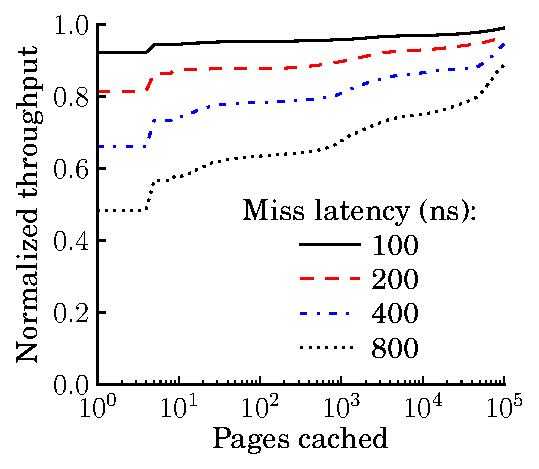
\includegraphics[width=.49\textwidth]{OLTP_eval/ReadPerformance_TATP.pdf}}
  \subfigure[TPCB]{\label{fig::ReadPerformance::TPCB}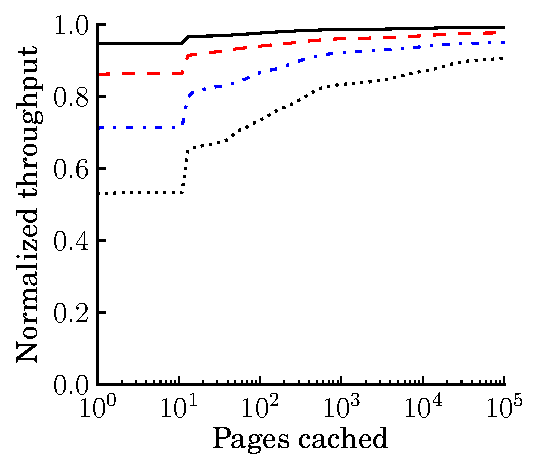
\includegraphics[width=.49\textwidth]{OLTP_eval/ReadPerformance_TPCB.pdf}}
  \subfigure[TPCC]{\label{fig::ReadPerformance::TPCC}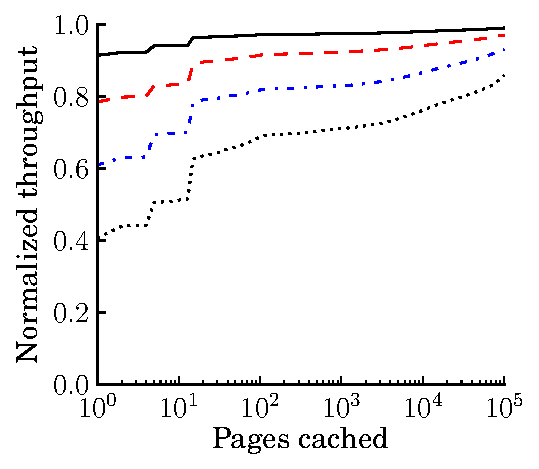
\includegraphics[width=.49\textwidth]{OLTP_eval/ReadPerformance_TPCC.pdf}}
%  \begin{subfigure}{0.32\textwidth}
%    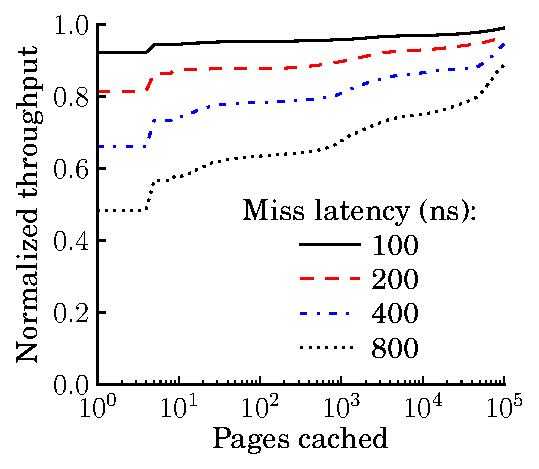
\includegraphics[width=\textwidth]{OLTP_eval/ReadPerformance_TATP.pdf}
%    \caption{TATP}
%    \label{fig::ReadPerformance::TATP}
%  \end{subfigure}
%  \begin{subfigure}{0.32\textwidth}
%    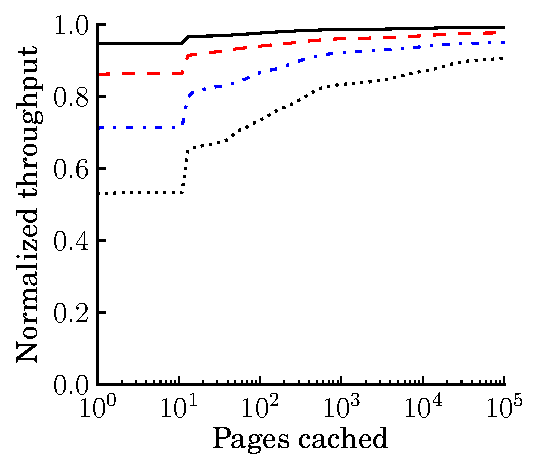
\includegraphics[width=\textwidth]{OLTP_eval/ReadPerformance_TPCB.pdf}
%    \caption{TPCB}
%    \label{fig::ReadPerformance::TPCB}
%  \end{subfigure}
%  \begin{subfigure}{0.32\textwidth}
%    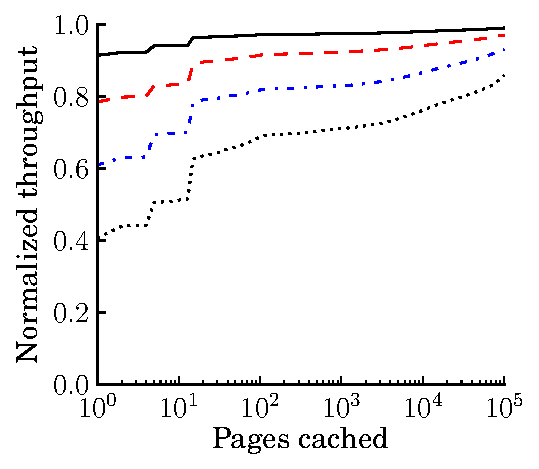
\includegraphics[width=\textwidth]{OLTP_eval/ReadPerformance_TPCC.pdf}
%    \caption{TPCC}
%    \label{fig::ReadPerformance::TPCC}
%  \end{subfigure}
  \caption{\textbf{Throughput vs NVRAM read latency.} 100ns miss latency suffers up to a 10\% slowdown over DRAM.  Higher miss latencies introduce large slowdowns, requiring caching.  Fortunately, even small caches effectively accelerate reads.}
  \label{fig::ReadPerformance}
\end{figure}

I create a timing model in Shore-MT from our memory traces.
Given traces, I perform cache analysis at page granularity, treating latches as page accesses and assuming a fully associative cache with a least-recently-used replacement policy (LRU).
Cache analysis produces an average page miss rate to each table.
I conservatively assume that every cache line access within an uncached page introduces an NVRAM stall, neglecting optimizations such as out-of-order execution and simultaneous multi-threading that might hide some NVRAM access stalls. 
The model assumes the test platform incurs a 50ns DRAM fetch latency, and adds additional latency to mimic NVRAM (for example, a 200ns NVRAM access adds 150ns delay per cache line).
I combine average page miss rate and average miss penalty (from lines/latch in table~\ref{table::AccessCharacteristics}) to compute the average delay incurred per latch event.
This delay is inserted at each page latch acquire in Shore-MT, using \InPlace, to produce a corresponding throughput.

Figure~\ref{fig::ReadPerformance} shows throughput achieved for the three workloads while varying the number of pages cached (horizontal axis) and NVRAM miss latency (various lines).
The vertical axis displays throughput normalized to DRAM-miss-latency's throughput (no additional delay inserted).
Without caching, throughput suffers as NVRAM miss latency increases, shown at the extreme left of each graph.
A 100ns miss latency consistently achieves at least 90\% of potential throughput.
However, an 800ns miss latency averages only 50\% of the potential throughput, clearly requiring caching.
Fortunately, caching proves remarkably effective for all workloads.
Each workload sees a spike of 10-20\% improvement for a cache size of just 20 pages.
As cache capacity further increases, each workload's throughput improves to varying degrees.
A cache capacity of 100,000 (or 819MB at 8KB pages) allows NVRAMs with 800ns miss latencies to achieve at least 80\% of the potential throughput.
While too large for on-chip caches, such a buffer might be possible as a hardware-managed DRAM cache \cite{QureshiSrinivasan09}.

\subsection{Analysis}
\label{sec:OLTP_eval:Reads:Analysis}
\begin{figure}
  \centering
  \subfigure[TATP]{\label{fig::Caching::TATP} 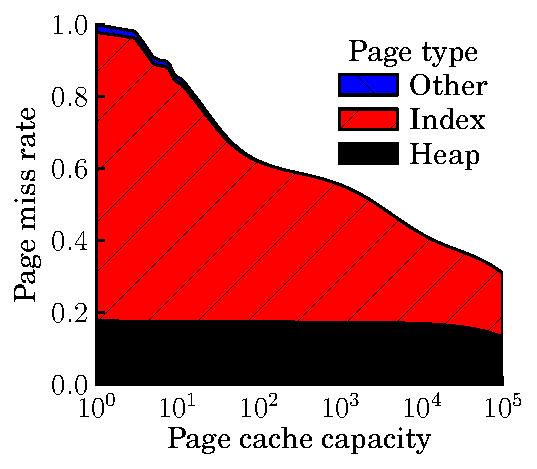
\includegraphics[width=.45\textwidth]{OLTP_eval/Caching_TATP.pdf}}
  \subfigure[TPCB]{\label{fig::Caching::TPCB}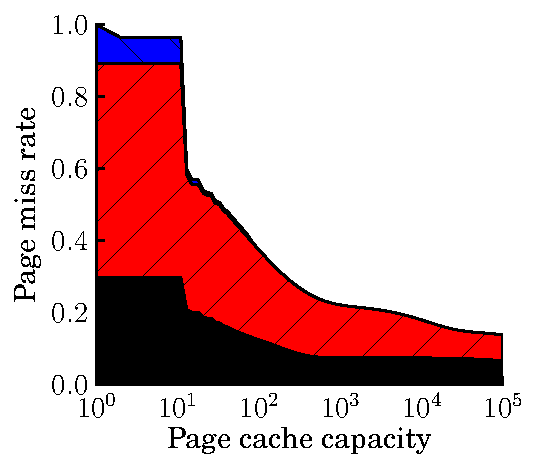
\includegraphics[width=.45\textwidth]{OLTP_eval/Caching_TPCB.pdf}}
  \subfigure[TPCC]{\label{fig::Caching::TPCC}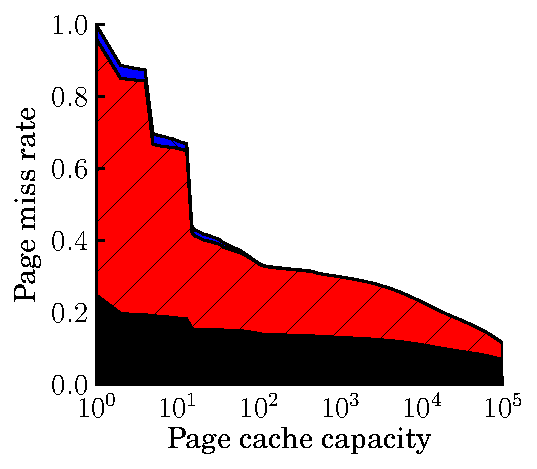
\includegraphics[width=.45\textwidth]{OLTP_eval/Caching_TPCC.pdf}}
  \caption{\textbf{Page caching effectiveness.} High level B+Tree pages and append-heavy store pages cache effectively.  Other pages cache as capacity approaches table size.}
  \label{fig::Caching}
\end{figure}

I have shown that modest cache sizes effectively hide NVRAM read stalls for our workloads, and further analyze caching behavior to reason about OLTP performance more generally.
Figure~\ref{fig::Caching} shows the page miss rate per page type (index, store, or other) as page cache capacity increases.
Each graph begins at 1.0 at the left -- all page accesses miss for a single page cache.
As cache capacity increases, workloads see their miss rates start to decrease between cache capacity of five and 20 pages.
TATP experiences a decrease in misses only in index pages, whereas TPCB and TPCC see a decrease across all page types.

While the behavior is specific to each workload, the results represent trends applicable to most databases and workloads, specifically, index accesses and append-heavy tables.
First, all workloads see a decrease in index page misses as soon as B+Tree roots (accessed on every traversal) successfully cache.
The hierarchical nature of B+Tree indices allows high levels of the tree to cache effectively for even a small cache capacity.
Additionally, TPCB and TPCC contain history tables to which data are primarily appended.
Transactions append to the same page as previous transactions, allowing such tables to cache effectively.
Similarly, extent map pages used for allocating new pages and locating pages to append into are frequently accessed and likely to cache.
The remaining tables' pages are accessed randomly and only cache as capacity approaches the size of each table.
In the case of TPCB and TPCC, each transaction touches a random tuple of successively larger tables (Branch, Teller, and Account for TPCB; Warehouse, District, Customer, etc. for TPCC).
This analysis suggests that various page types, notably index and append-heavy pages, cache effectively, accelerating throughput for high-latency NVRAM misses with small cache capacities.

\textbf{Bandwidth.}
\begin{table}
  \centering
  \begin{tabular}{l l}
    \hline
    Workload & Bandwidth (GB/s) \\
    \hline \hline
    TATP & 0.977 \\
    TPCB & 1.044 \\
    TPCC & 1.168 \\
    \hline
  \end{tabular}
  \caption{\textbf{Maximum required NVRAM read bandwidth.} Workloads require approximately 1 GB/s NVRAM read bandwith, well below technology limits.}
  \label{table::ReadBandwidth}
\end{table}

Finally, I briefly address NVRAM read bandwidth.
For a worst-case analysis, I assume no caching.
Given the average number of cache line accesses per page latch, the average number of page latches per transaction, and transaction throughput (taken from Section~\ref{section::Persists}), I compute worst-case NVRAM read bandwidth for each workload, shown in Table~\ref{table::ReadBandwidth}~
The considered workloads require at most 1.168 GB/s (TPCC).
Since this is substantially lower than expected NVRAM bandwidth and caching reduces the required bandwidth further, I conclude that NVRAM read bandwidth for persistent data on OLTP is not a concern.

\subsection{Summary}
\label{sec:OLTP_eval:Reads:Summary}
NVRAM presents a new storage technology for which modern database systems have not been optimized.
Increased memory read latencies require new consideration for database caching systems.
I show that persistently stored data for OLTP can be cached effectively, even with limited cache capacity.
I expect future NVRAM software to leverage hardware caches, omitting software buffer caches.
Next, I turn to write performance for storage management on NVRAM devices.
